\chapter{Topic Classification}
\label{sec:classification}
\chaptermark{Topic Classification}
In this chapter we examine locality and topic information in the context of topic classification of speech.   We wish to highlight the importance of locality as pertains to the topics of informal speech but also to highlight the error robustness of the topic signal.  We demonstrate a much stronger  relationship between keyword retrieval metrics and Topic ID Error than between that and word error rate (WER).  This analysis leads us to focus in  subsequent chapters on more specific models of topic information for keyword-based retrieval.

\section{Locality in Informal Speech}
\label{sec:topicDrift}
We first examine the location-sensitive nature of topic information in spoken documents.  By a simple initial experiment we can show that information corresponding to the topic label for the available topic-annotated spoken corpora tends to be concentrated towards the beginning of documents (cf. Table~\ref{ch3quartiles}).  Building on this result we then present a model for topic locality within a bag-of-words framework.  Applying our model to the classification task, effectively ignoring irrelevant words later in documents we can reduce the error rate by up to 50\% (cf. Figure~\ref{ch3main}).

\begin{figure}[ht]
\centering
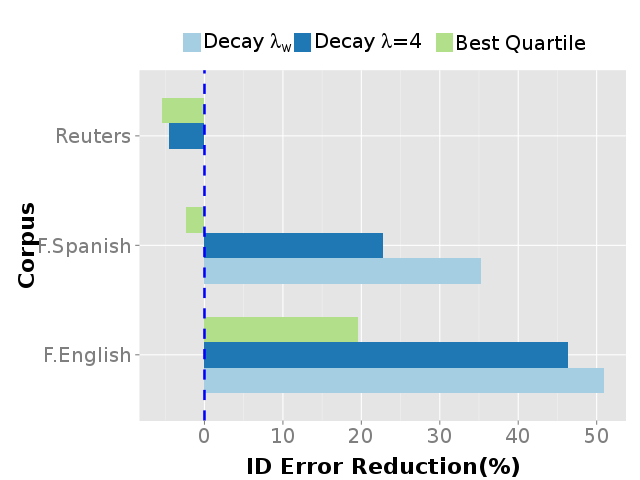
\includegraphics[width=0.6\textwidth]{locality2.png}
\caption[Topic ID Error reduction for location-dependent features]{\label{ch3main} Topic ID Error reduction for location-dependent features}
\end{figure}

%Decaying cache models
Presumably topic location dynamics is domain-specific, so we contrast informal speech with newswire text, where we do not expect our assumptions about speech to hold.  We perform the classification task using the Fisher English and Spanish human transcripts and the Reuters RCV1 text categorization corpus\cite{lewis2004}.  

Rather than building bags-of-words from each document in its entirety, we restrict each document vector to a specific quartile.  If the topic signal is evenly distributed, we do not expect the performance on one quartile to be significantly better or worse than another.  By the first quartile, for example we mean that will construct features for both training and testing classifiers from only the first 25\% of words (by position) in each document.  So for a document with 100 words, we would only count words 1 to 25 for the first quartile test, words 26-50 for the second 25\%, and so on.   

\begin{table}[t]
\centering
\vspace{2mm}
%\centerline{
\begin{tabular}{c|c|c|c|c|c} \toprule
\textbf{Corpus} & \textbf{All} & \bf 0-25\% & \bf 25-50\%  & \bf 50-75\% & \bf 75-100\% \\
\midrule \midrule
Reuters & \textbf{20.1} & 23.5 & 21.9 & 21.7 & 21.2 \\
Fisher English & 11.2 & \bf 8.9 & 24.3 & 38.5 & 43.6 \\
Fisher Spanish & \textbf{25.0} & 25.6 & 34.7 & 42.1 & 48.3 \\\bottomrule
\end{tabular}
\caption[Topic ID Error rates by quantile]{\label{ch3quartiles} {ID Error rate (\%) observed when training and testing on data by quartile.}}
\end{table}

Table~\ref{ch3quartiles} shows the results of this simple test using a Naive Bayes classifier as described in \cite{wintrode2013}.   Not surprisingly, performance on the Fisher corpora, in which participants are asked to call in and are prompted to talk about a particular topic (which is used as ground truth for the task), is significantly higher on the first quartile, roughly as good as using the entire conversation, and significantly lower on the remaining 75\%.   Conversely, the Reuters corpus does not exhibit any obvious location dependence, as we expected.


% what picture to show? --- demonstrate visually impact of locality
%We can formalize this phenomenon by assuming generalize this result by explicitly modeling topic location we can further improve topic identification.

\subsection{Static Topic Drift}
In the general case, there is no reason to believe an arbitrary division such as a quarter of a document should capture within-document topic locality. Instead we propose to model the observed \textit{topic drift}, in which the contribution of individual occurrences of words to the effective topic signal (as measured on the identification task) decreases over the course of the document.

We first model drift by supposing a global decay rate for all words in the vocabulary.  This idea is similar in spirit to decaying cache language models (cf. \cite{clarkson1997}).   Within our framework we can also learn word-specific decay rates for each word using a minimum classification error (MCE) training framework.  With the dynamic approach, for the informal corpora we are able to cut ID errors in half from the full bag-of-words baseline.

To apply a decay model to the word counts of a document when computing a bag-of-words vector, for each word type we apply a decay function to each token instance evaluated at position $p$ and with decay rate $\lambda$ and sum over tokens.  So the count $c_w$ for a word $w$ in a document of $|D|$ words is given as:

\begin{align}
c_{w} &= \sum_{i=1}^{|D|}{d\left(p=\frac{i}{|D|},\lambda\right) \cdot I_{w}(w_i)}
\label{eqStatic}
\end{align}

$I_w(w_i)$ is an indicator function whose value is 1 where $w_i=w$ and 0 otherwise.

We considered three possible decay functions, exponential, gaussian, and linear (cf. Eqns.~\ref{eqExp},\ref{eqGauss},\ref{eqLin}) over the range $[0,1]$.   Examples of each for different $\lambda$ values are shown in Figure~\ref{ch3DecayExample}.
\begin{align}
  d_{exp}(p, \lambda) &= exp \left ({ -\lambda \cdot p }\right ) \label{eqExp} \\
  d_{gauss}(p, \lambda) &= exp \left ({ -\frac{\lambda^2 \cdot p^2}{2} }\right) \label{eqGauss} \\
  d_{lin}(p, \lambda) &=  \left\{
     \begin{array}{lr}
       1 - \lambda \cdot p & : p \in [0,1]\\
       0 & : p \notin [0,1]
     \end{array}
   \right. \label{eqLin}
\end{align}

\begin{figure}[t]
		\centering
		\subfloat[Exponential\label{subfig-1:exp}]{%
          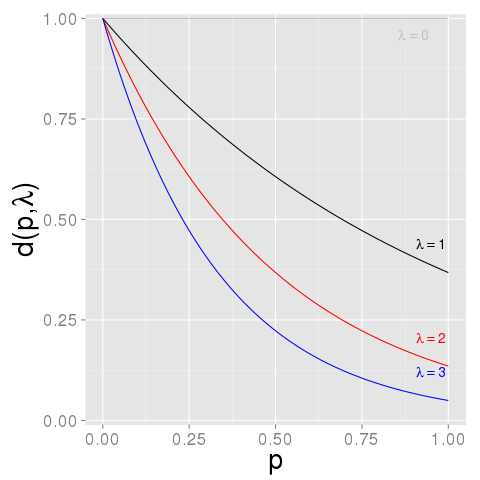
\includegraphics[width=0.32\textwidth]{graphs/ch3/example-exp.png}
        }
		\subfloat[Gaussian\label{subfig-1:gauss}]{%
		    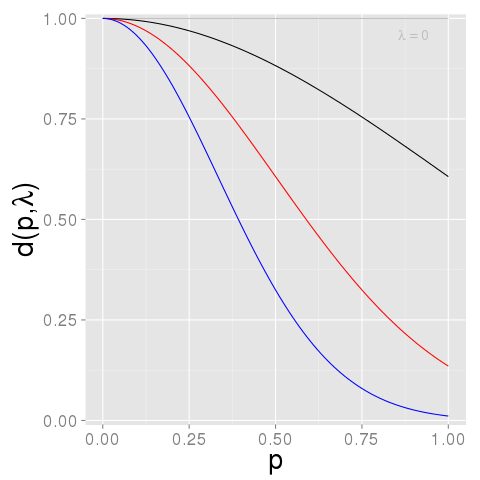
\includegraphics[width=0.33\textwidth]{graphs/ch3/example-gauss.png}
		}
        \subfloat[Linear\label{subfig-1:linear}]{%
          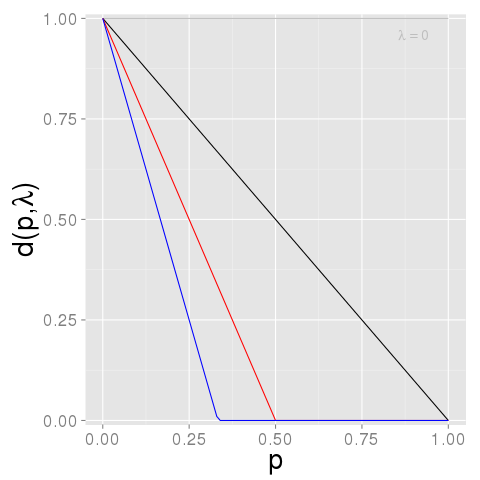
\includegraphics[width=0.32\textwidth]{graphs/ch3/example-lin.png}
        }
      \caption[Decay function behavior]{Decay function behavior for selected $\lambda$.\label{ch3DecayExample}}
\end{figure}

In the static case, we swept values for $\lambda$ from 0 to 5, where 0 corresponds in each case to the unweighted baseline counts and 5 being the point after which we observed no additional benefit or degradation in performance.   The linear decay generally performed poorly, regardless of $\lambda$.

The best results of the static model are listed in Table~\ref{tab:drift}.  Again we see that modeling drift has no significant effect on performance on the Reuters text corpus whereas for the informal speech, the exponential decay with $\lambda=4$ decreases ID error over the bag-of-words baseline by 46\% and 23\% relative for English and Spanish respectively.  Interestingly enough, evaluating $d_{exp}(p=0.25, \lambda=4)=0.37$ shows that words after the first quartile are discounted by at least 63\%, but do contribute a small amount to the overall weighted word counts.

\subsection{Word-specific Topic Drift}

While the static model is effective in applying location-dependent weighting to all words uniformly, our dynamic model supposes that specific words are more or less sensitive to their position in the document with respect to the Topic ID task.  We simply extend Equation~\ref{eqStatic} with per-word decay rate $\lambda_w$.

\begin{align}
c_{w} &= \sum_{i=1}^{|D|}{d\left(p=\frac{i}{|D|},\lambda_w\right) \cdot I_{w}(w_i)}
\label{eqDynamic}
\end{align}

We optimize per-word weights $\lambda_w$ using a Minimum Classification Error (MCE) discriminative framework.  We configure our Naive Bayes classifier to compute a score $S(t|D)$ for each document $D$ against each topic $t$.  We can compute a loss function based on a misclassification measure $M(D)$ and maximize the difference between the score for the correct topic $t_C$ and the highest scoring incorrect hypothesis $t_I$.

\begin{equation}
M(D)=S(t_I|D)-S(t_C|D)
\end{equation}

We compute the partial derivative and update equations for a gradient-descent optimization of $M(D)$ over $\lambda_w$.  These partial derivatives, with the score function $S(t|D)$ given by a Naive Bayes classifier based on our modified counts $c_w$, can be expressed terms of the decay functions.    A full derivation for $\lambda_w$ updates is provided for reference in Appendix~\ref{sec:mceAppendix}.  

Allowing the gradient descent to run to convergence reduces the error rate further over the static model.  the overall results are listed in Table~\ref{tab:drift}.  Learning $\lambda_w$ for an exponential decay ($d_{exp})$, outperformed the best static decay model, which was also exponential, with a fixed decay reate of $\lambda=4$.  These numbers correspond to the error rate reductions highlighted a the start of the chapter (Figure ~\ref{ch3main}). A representative run of the MCE training, contrasting the loss function on both train and test data with the observed error metrics on the test data is given in Figure~\ref{ch3converge}.  %A complete table of results is given in Appendix~\ref{sec:idResults}.

If we look at the words with the highest learned decay rate (Table~\ref{ch3words}) on the Spanish corpus, two things stand out.  High decay rates are learned on both information rich words (\textit{guatemala, méjico, boston}) and typical stopwords (\textit{hm, oh, sí}).  Given the corpus, where participants who do not know one another call into a switchboard at LDC to be recorded, this makes sense.  The place names, while information rich, typically occur during the chit-chat at the beginning of the conversation, but are in fact irrelevant to the topic.


% good illustration of MCE
\begin{figure}[t]
	\centering
	\null\hfill
	\subfloat[\label{ch3converge} Error measures on learning $\lambda_w$.]{
      \raisebox{-2.3cm}{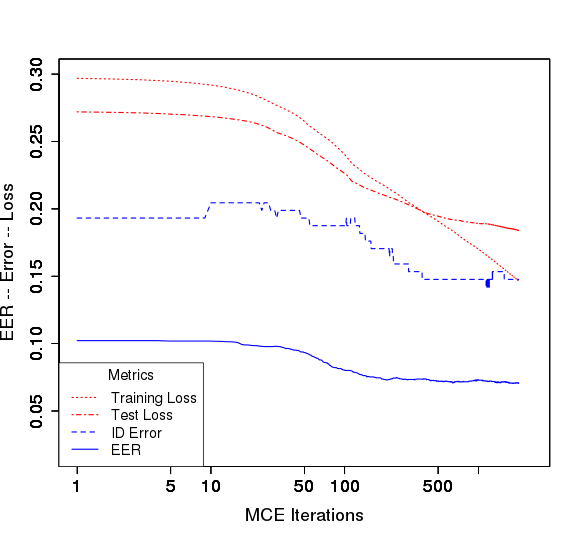
\includegraphics[width=0.38\textwidth]{graphs/ch3/mce-error.png}}
	}
	\hfill
	\subfloat[\label{ch3words} {Highest decay-rate words}] {
		\scriptsize
		\begin{tabular}{c r c r} \toprule
		\multicolumn{4}{c}{\textbf{Word  (Decay Rate)}} \\
		\midrule \midrule
		hm & 10.44 & boston & 8.31 \\
		guatemala & 10.19 & muy & 8.28 \\
		asunción & 9.95 & más & 8.16 \\
		acá & 9.85 & chicago & 8.13 \\
		oh & 9.09 & miércoles & 8.09 \\
		sí & 9.01 & puerto & 8.06 \\
		uh & 8.86 & me & 8.04 \\
		méjico & 8.66 & um & 7.96 \\
		ajá & 8.52 & es & 7.86 \\
		bonito & 8.40 & uhum & 7.83  \\
		\bottomrule\\[1ex]
		\end{tabular} %\vskip0.1cm
	}
	\hfill\null
	\caption[MCE training]{MCE training measures} 
\end{figure}

\begin{table}[htbp]
\centering
\begin{tabular}{c|c|c|cc} \toprule
\bf Corpus & \bf $\lambda$ & \bf Iterations & \multicolumn{2}{c}{Error} \\
           &               &                &  $d_{gauss}$ & $d_{exp}$ \\
\midrule
Reuters & 0 & -  &  -  &  20.1\% \\          
        & 1 & -  &  20.5  &  20.5\% \\          
English & 0 & - &  & 11.2\% \\ %\cline{2-9}
        & 4 & - & 7.3\% & 6.0\% \\
        & $\lambda_w$ & 2000 & 5.7\% & 5.5\% \\
Spanish & 0 & - & - & 25.0\% \\
        & 4 & - & 19.9\%  & 19.3\% \\
        & $\lambda_w$ &  2000 & 15.3\% & 14.2\% \\ %\cline{2-9}
\bottomrule
\end{tabular}
%\end{center}
\caption[Topic ID error for feature decay models]{\label{tab:drift} Topic ID error by corpus for feature decay models.}
\end{table}

% should probably put complete results somewhere....

As we have seen, topic information can be highly localized, and we argue that the phenomenon we have observed and modeled lend support to the consideration of decaying cache style language models.   We will now turn our attention to topicality and its relation to speech recognition errors.  Although topics are highly localized, the information is extremely robust to a high number of ASR errors.


\section{Word Error Robustness}

As we discussed in Chapter~\ref{sec:bkg}, topic classification  performance on speech recognition output is remarkably insensitive to changes in word error rate (WER) over a broad range of reasonable operating points.

In the rest of this chapter we present and elaborate on work originally presented in \cite{wintrode2014} to demonstrate how errors on information-rich keywords are more predictive of classification performance than WER.  These experiments motivate subsequent chapters where we focus on using topic information to target improvement of KWS accuracy. % which in a virtuous cycle, can improve topic ID performance

The reason why classification performance is insensitive to WER is fairly intuitive, particularly given the work on feature selection for classification (cf. \cite{yang1997}, \cite{hazen2007}).  Feature selection experiments generally indicate that using only the most discriminative words results in equal or better performance than using the entire vocabulary.   WER by contrast is computed over all words in the vocabulary, as we mentioned in Chapter 2.  Feature selection results imply that most words are uniformly distributed between positive and negative training examples (and thus uncorrelated with the topic label).  We would assume that the insensitivity of classification error to WER changes indicates that errors on these `uninteresting' words are also evenly distributed between positive and negative training examples.  In other words, most of the change in WER is related to these words that have no relevance to the topic content.

We replicated the analysis in \cite{yang1997} and demonstrate this effect on the Fisher Spanish 25-topic classification task described previously.  By selectively increasing the vocabulary used for classification based on the $\chi^2$ statistic, we achieve the best error rates using only a small fraction (2-3\%) of the vocabulary (Figure~\ref{ch3Chi2}).  We test a wider range of error conditions using keyword search metrics, by narrowing our focus to the top 1000 words, according to the $\chi^2$ statistic.

%This suggests that very \textit{limited vocabulary} solutions may be used in a high volume setting, and one need not extract a large bag of all possible word types.

% make sureto place line at 1000, and include 30000 in graph....
% information in 10 % of vocab

\begin{figure}[t]
\centering
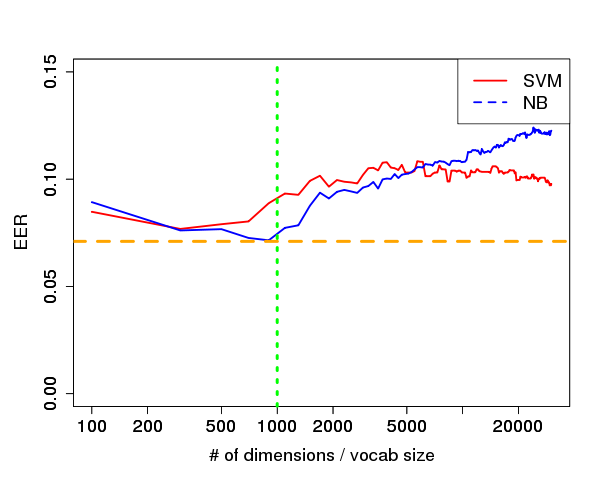
\includegraphics[width=0.65\textwidth]{graphs/ch3/chi2-poster.png}
\caption[Effect of feature selection on Fisher Spanish classification]{Effect of $\chi^2$ feature selection on the Fisher Spanish classification task.\label{ch3Chi2}}
\end{figure}
% ASR output, orange line is SVM EER on human transcripts

\subsection{ASR Models}

To capture the relationship between ASR errors and topic classification performance, we first decode the Fisher Spanish with a range of acoustic and language models of varying complexity.  We contrast the performance of the actual ASR system with randomly generated word errors induced on the ground truth but covering a wider range.  To increase the amount of error further (without simulation and using the same training data) we also construct limited vocabulary keyword spotters for the same task.

We first use the Kaldi speech recognition toolkit \cite{kaldi} to train a 45K word Spanish ASR system on only the 14 hour Spanish Call Home data \cite{callhome}.  The vocabulary and pronunciations are also restricted to the Call Home lexicon.  This translates to out-of-vocabulary (OOV) rates of 47\% (types) and 5.7\% (tokens). In fact, roughly 10\% of our top keywords were OOV.

For all acoustic model training, we use 13-dimensional perceptual linear predictive (PLP) features.  These PLPs are used to train both speaker-independent and speaker-adapted triphone models using typical state-clustered HMM's with GMM output densities (denoted \textbf{GMM} in subsequent figures).  We also trained Subspace GMM's \cite{povey2010} (SGMM) from the PLP's as well (denoted \textbf{SGMM}).  The SGMM parameters can also be boosted with a maximum mutual information (MMI) criterion.  All models use a trigram language model estimated on the Call Home transcripts, and the individual data points for a specific acoustic model reflect varying the language model weight during decoding (cf. Figure~\ref{ch3WER}).

We also use Kaldi's CPU-based deep neural net (DNN) acoustic models in a hybrid HMM-DNN configuration \cite{vesely2013} (denoted \textbf{DNN}).  For small training sets ($\sim$10hrs) Kaldi uses a smaller network configuration of only 2 hidden layers and 879 input and output dimensions.  The DNN features had little impact on the full vocabulary ASR results, but large impact on the keyword spotting results, as we will see.

Figure~\ref{ch3WER} shows just how little effect a large change in WER has on topic classification, consistent with previous work.  The dashed lines indicate the EER of topic classification training and testing on human transcripts with an SVM (7.1\%) or Naive Bayes (12.2\%) classifier.  We see that a 9.4\% difference in WER still falls within the bounds of performance on manual transcripts.
% illustrates just how irrelevant WER is, on smaller scales
\begin{figure}[ht]
\centering
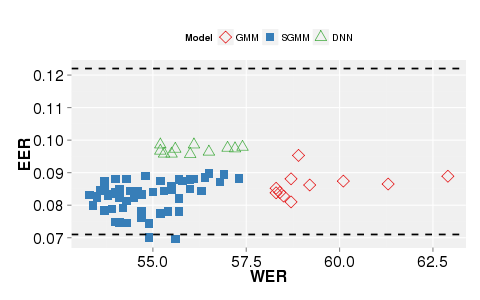
\includegraphics[width=0.7\textwidth]{graphs/ch3/svm-wer.png}
\caption[Effect of WER on Fisher Spanish EER]{Relation between WER and topic detection EER for Fisher Spanish\label{ch3WER}}
\end{figure}

To understand the significance of this performance range we simulate word errors over the entire range from 5 to 95\% WER by randomly inducing either substitutions or deletions in the ground truth transcripts.  The full vocabulary systems tended to exhibit roughly twice as many substitution errors as deletions.  To induce a 35\% WER system, each word  in the true transcripts had a 35\% change of being modified, and if chosen, a 33.3\% change of being deleted or a 67\% chance of being replaced with an incorrect word.  Word substitutions were selected uniformly from the vocabulary.  In an actual ASR system, substitutions are often `sounds-like' errors, but this distinction is lost when computing WER.  For comparison we also simulated systems over the same WER range but entirely with deletions.

\begin{figure}[t]
\centering
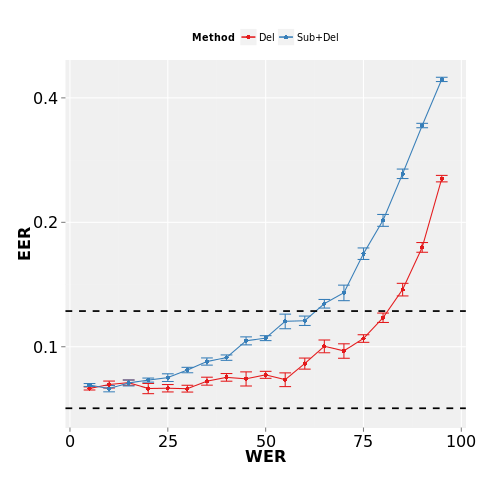
\includegraphics[width=0.6\textwidth]{graphs/ch3/gen-wer.png}
\caption[Simulated WER and Fisher Spanish EER]{Simulated WER and topic detection EER for Fisher Spanish\label{ch3genWER}}
\end{figure}

Figure~\ref{ch3genWER} compares topic classification performance on the simulated errorful transcripts at 5\% WER intervals.  We ran 10 trials for each type of error induction method at each WER point, and the standard error over the trials are indicated by the error bars.  Figure~\ref{ch3genWER} is plotted with the EER on a log scale for legibility.   For the deletion-only systems, we do not see changes in classification EER larger than a single standard deviation until WER exceeds 50\%.  For the mixed error simulation (Sub+Del) significant changes are observed at lower WER (higher accuracy) systems.

The difference between the two simulations makes intuitive sense in terms of the classification task.  Deletion errors suggest missing but not misleading evidence for the conversation topic.  If we place the actual ASR systems on the same graph with the simulations (cf. Figure~\ref{ch3genWERzoom}) we observe that despite exhibiting a 2 to 1 substitution to deletion ratio, the true ASR errors induce topic classification performance closer to the deletion-only simulation.  For example, in the a system with 65\% WER, approximately 2500 out of 291000 substitution errors differed only by the addition or subtraction of the plural `s' at the end of the word - e.g. \textit{matrimonio} vs. \textit{matrimonios}.   A random substitution is much more likely to result in a topically unrelated word.

\begin{figure}
\centering
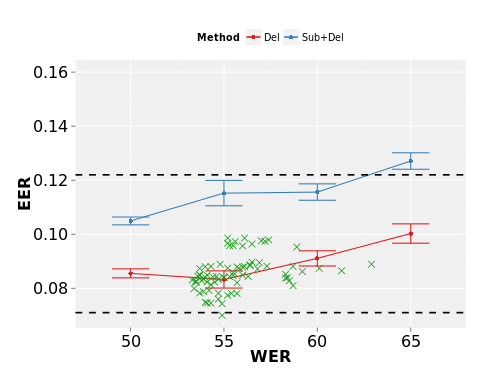
\includegraphics[width=0.7\textwidth]{graphs/ch3/gen-wer-zoom.png}
\caption[Simulated WER and Fisher Spanish EER]{Simulated WER and topic detection EER for Fisher Spanish.  Actual ASR systems in green.\label{ch3genWERzoom}}
\end{figure}


\subsection{Keyword Spotting Models}

To present an additional perspective on where topic content begins to be lost due to speech recognition errors we also built a limited vocabulary keyword spotting system for the top 1000 keywords.  In most cases the keyword spotting system does \textit{not} permit classification performance on par with the human transcript baseline.  By evaluating the higher error system in terms of keyword retrieval metrics, rather than aggregate WER, we are better able to identify which errors from the ASR system on which to focus subsequent efforts for improvement.  In our analysis, ranked retrieval metrics, particularly the area under the keyword recall-precision curve (AUC), are better predictors of the ability to perform topic classification.

We construct a keyword spotting system from standard HMM-based ASR tools, again with the Kaldi framework.  Our training corpus is the same as the full vocabulary system, however we assume that only instances of the top 1000 keywords are annotated for acoustic training.  The remaining speech is mapped to a filler word.  The language model, if useful at all, models the transition from filler word to the keywords and vice versa.  However, the best retrieval performance was observed with a minimal language model scaling factor, indicating the acoustic model contained most of the useful information.  

The keyword spotting follow the same training procedure as for the full vocabulary system so we obtain results for GMM, SGMM, and DNN output density models on HMM states (i.e. context-dependent triphones).   Further details of the keyword spotting architecture can be found in \cite{wintrode2014}.

\subsection{Results}
In contrast to the full-vocabulary systems, the keyword spotting models do not exhibit Topic ID performance on par with the transcript baseline, \emph{except for the DNN-based models} (cf. Table~\ref{ch3KWSpotting}).  Rather than be disappointed by these results, we use this opportunity to look at the retrieval results and identify causes for the degradation.

The most noticeable difference between the DNN and GMM models is the increase in recall.  On average, the DNN models recalled nearly \textbf{twice as many} keyword instances as the other models.  By contrast, the GMM keyword spotters had the highest precision on the search task but the lowest overall topic performance.  We may conclude that a higher false alarm rate (low precision) does not by itself inhibit topic classification performance.

\begin{table}[t]
\centering
\begin{tabular}{l||c||c|c|c|c}\toprule
\multicolumn{6}{c}{Keyword Spotting Systems}\\\midrule
Acoustic Model & EER & Recall & Prec. & MAUC & TWV\\\midrule
GMM & 0.39 & 0.084  & \bf 0.641 & 0.043 & \bf -0.004 \\
SGMM & 0.29 & 0.172 & 0.545 & 0.079 & -0.012 \\
\textbf{DNN} & \textbf{0.12} & \textbf{0.379} & 0.338 & \textbf{0.154} & -0.038 \\\midrule
%\textit{Transcripts (V=30k)} & 1.0 & 1.0 & 1.0 & 0.12 \\ \midrule
\multicolumn{6}{c}{Full Vocabulary ASR}\\\midrule
%Model & EER & Recall & Prec. & MAUC & TWV\\\midrule
GMM & 0.09 & 0.278 & 0.464 & 0.395 & 0.342 \\
SGMM & 0.08 & 0.318 & 0.482 & \bf 0.428 & \bf 0.384 \\
DNN & \bf 0.07 & 0.269 & 0.458 & 0.433 & 0.384 \\ \bottomrule
%\textit{Transcripts (V=1k)} & 1.0 & 1.0 & 1.0 & 0.07 \\
\bottomrule
\end{tabular}
\caption[Topic ID EER and ranked keyword retrieval accuracy ]{\label{ch3KWSpotting} Naive Bayes Topic ID EER and keyword retrieval performance for various metrics.  Paired t-test gives $p < 2\times10^{-16}$ between different acoustic model EER results.}
\end{table}

Based on the recall and precision of the keyword spotters, (top portion of Table~\ref{ch3KWSpotting}) it is tempting to argue that recall by itself is sufficient for reasonable Topic ID performance.  However, the ranked retrieval performance reveals something more nuanced.   

Figure~\ref{auc1} shows the keyword spotting retrieval results in terms of the mean search AUC (MAUC) of all keywords plotted against EER.   The keyword spotting systems, even with DNN features, are at least 50\% lower in terms of search accuracy than full-vocab ASR performance.  The DNN system, however is twice as accurate in terms of ranked retrieval than all other keyword spotters.  

Ranked retrieval metrics reflect the order of results.  Higher AUC implies that correct keyword detections are more likely at the top of the term detection results.  As we generate counts for Topic ID from the results, detections at the top contribute more to our bag-of-words model.  We conjecture that for the DNN models, retrieval is good enough, given sufficient recall of topic-relevant words, that false alarms that obscure the topic signal do not occur high up in the result list. 


\begin{figure}[t]
\centering
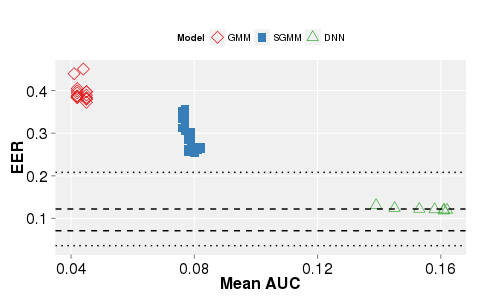
\includegraphics[width=0.75\linewidth]{graphs/ch3/nb-mauc-eer.png}
\caption[Effect of keyword accuracy on Topic EER]{\label{auc1} Effect of keyword accuracy on Topic EER.  Dashed lines indicate Naive Bayes and SVM performance on human transcipts.   Dotted lines indicate standard deviation across topics on human transcript performance.}
\end{figure}


\section{Conclusion}

In this chapter we considered topic information from the perspective of the topic classification task.   We have drawn two conclusions, first, topic information is sensitive to location, that is, a bag-of-words model that ignores location does not accurately model topic information spoken documents (with respect to classification).  Secondly, we have examined the robustness of topic information in speech with respect to recognition errors.  We have argued that improving keyword retrieval is more relevant to improving topic classification than is optimizing word error rate.  Thus in subsequent chapters, we will be more interested in developing techniques that improve KWS performance on speech, not just WER.

